\section{Extending VRAE to Uneven Samples}
\label{proposal}

Based on the effectiveness of deep stochastic models we propose two VRAE extensions that can properly handle dimensionality reduction of light curves with unevenly-sampled time series. The first model is a natural extension from VRAE that includes the time of the signal while the second model adds the scale information into the dimensionality reduction task.

\subsection{Problem Setup}

\begin{figure}[t!]
    \centering
    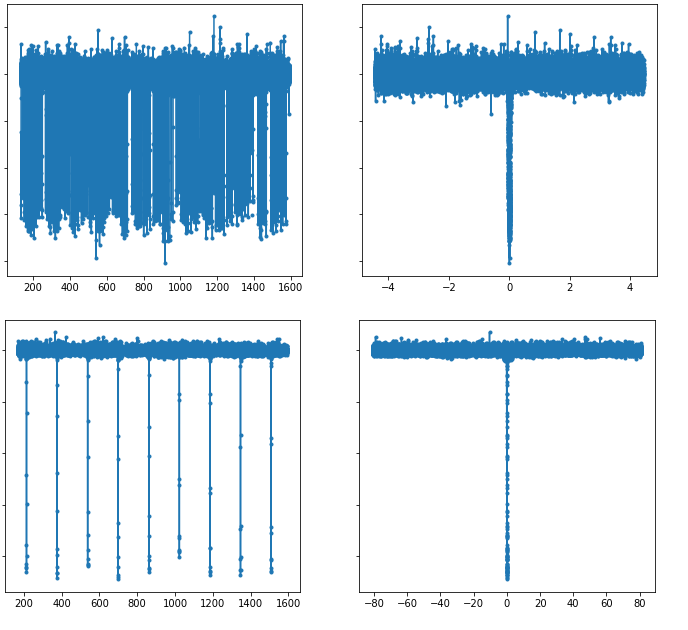
\includegraphics[width=0.95\textwidth, height=6cm]{imgs/LC_ex.png}
    \caption{Examples of light curves on Kepler mission. First column correspond to 4 years measurements with sampling rate of half an hour, while the second column correspond to the folded transit.}
    \label{fig:lc_ex}
\end{figure}

Consider a dataset $X = \{x^{(1)}, x^{(2)}, \ldots, x^{(N)}\}$, of $N$ input patterns $x$ distributed according to a unknown probability distribution $p(x)$. These inputs pattern are vectors of variable length, $x^{(i)}= (x^{(i)}_1, x^{(i)}_2, \ldots, x^{(i)}_{T_i})$, where $x^{(i)}_j \in \mathbb{R}$ represent the $j$-th observation of the time series $x^{(i)}$ of length $T_i$. Let ${t}^{(i)}_j$ be the timestamp when the $j$-th observation was obtained for data $i$. Furthermore, we define the time interval, or \textit{delta time}, for each observation: $\delta^{(i)}_j = t^{(i)}_j - t^{(i)}_{j-1} $, with $\delta^{(i)}_0 = 0 \ \forall i$.

This paper focuses on the transit-shape domain objects over the light curve $x^{(i)}$, in order to recognize patterns of exoplanets orbiting its host star. An example is shown on Figure \ref{fig:lc_ex}.

\subsection{VRAE for Unevenly-Sampled Time Series}

\begin{figure}[!t]
    \centering
    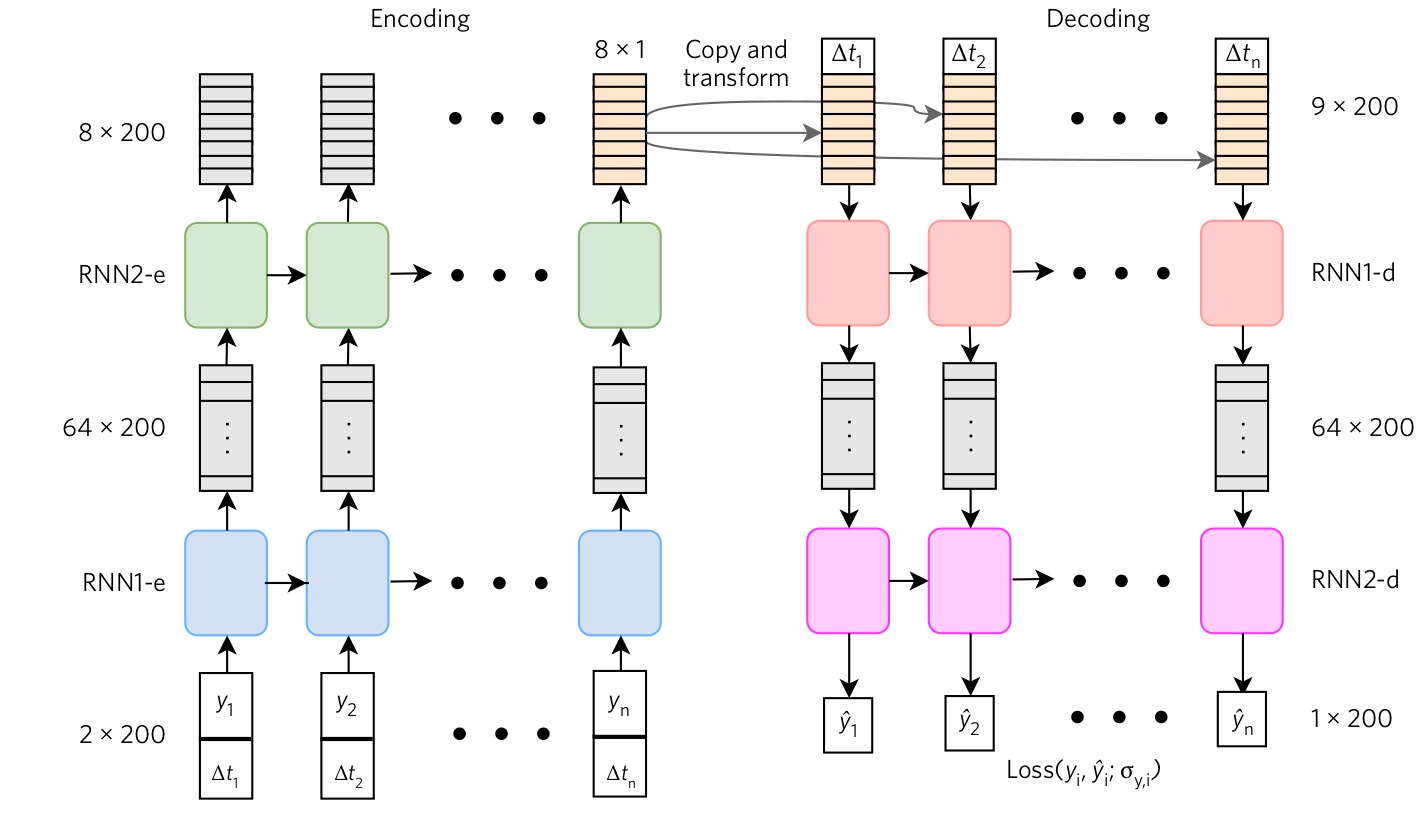
\includegraphics[width=0.9\textwidth]{imgs/BNaul_model.png}
    \caption{Diagram of the RAE$_t$ architecture for irregularly sampled time series data proposed by \citep{naul2018recurrent}. The sequence is processed by recurrent layers to produce a final fixed-length embedding with a single fully connected layer on last state. The decoder first repeats the fixed-length embedding $T_i$ times, and then appends the delta times ($\delta$, on figure $\Delta t$). The sampling times are passed to both the encoder and decoder; this is for determine the points at which the function should be evaluated.}
    \label{arch:bnaul}
\end{figure}

A Variational Auto-Encoder (VAE), like any Auto-Encoder architecture, is composed of a tangled encoder and decoder models trained on a unsupervised scenario\footnote{Unsupervised refers to the fact that no labels are used as inputs to the model.}. The encoder model $q_{\phi}(z|x)$, with parameters $\phi$, codifies the input pattern $x$ to a latent variable $z$, and the decoder model $p_\theta(x|z)$, with parameters $\theta$, reconstructs the input pattern from the codification $z$. The objective of the model is to maximize a (variational) \textit{lower bound} $\mathcal{L}(\theta,\phi; x^{(i)})$ of the log-likelihood $\ell(\theta,\phi; D)$ \citep{kingma2013auto}. For example, for an input pattern $x^{(i)}$ we have
\begin{align} \label{eq:basic_obj}
\ell \geq & \mathcal{L}(\theta,\phi; x^{(i)}) = \mathbb{E}_{q_{\phi}(z |x^{(i)})}\left[\log{p_{\theta}(x^{(i)},z)} -\log{q_{\phi}(z|x^{(i)})}  \right] \, \notag \\
    & \mathcal{L}(\theta,\phi; x^{(i)}) =  \mathbb{E}_{q_{\phi}(z |x^{(i)})}\left[ \log{p_{\theta}( x^{(i)} | z )}\right] - D_{\mbox{\tiny KL}}\left( q_{\phi}(z | x^{(i)}) || p_{\theta} (z)  \right) \, ,
\end{align}
where the first term of $\mathcal{L}$ is related to the expected reconstruction likelihood and the second enforces the consistency between the posterior obtained by the encoder $q_{\phi}(z|x)$ and some prior $p_\theta(z)$ (i.e., KL divergence). In the standard VAE, the distribution $q_{\phi}(z|x)$ is typically a normal $\mathcal{N}(\mu(x),\sigma(x))$ where $\mu(x), \sigma(x)$ are modeled by neural networks, while the common choices of $p_\theta(z)$ leads a KL divergence that can be integrated analytically. However, the first term of $\mathcal{L}$ needs to be approximated with the so-called \emph{re-parametrization trick}: $\hat{z} = \mu + \sigma \cdot \epsilon$, with an auxiliary noise variable $\epsilon\sim \mathcal{N}(0,1)$.

The shallow (fully connected) VAE for light curves proposed by \citep{woodward2019generating} could be extended to adapt RNN models into the encoder $q_{\phi}(z|x)$ and decoder $p_\theta(x|z)$ as a VRAE model.
However, to adapt the model for being used with unevenly-sampled light curves, we need the time intervals ($\delta$) as an extra input channel. 
To do this we follow the idea of the RAE$_t$ architecture proposed by \citep{naul2018recurrent} (shown in Figure \ref{arch:bnaul}), which adds the time information in both encoding and decoding sections of the autoencoder.
The proposed extension is called \textbf{VRAE$_t$} model (VRAE \textit{plus} time information). This model could be expressed by the encoder $q_{\phi}(z|x,\delta)$ and the decoder $p_\theta(x|z,\delta)$ which have the time information $\delta$ of every observation on the time series $x$ as an extra input signal.

%ventajas de VAE sobre AE (smooth light curve e independientes):
The motivation behind the variational extension is that the generative (stochastic) model learns a latent variable with smoother transitions, meaning that their latent space must be continuous \citep{kingma2013auto}.
%conectar con esto: (para entender que el modelo puede ser visto como un denoising) -- aprende los patrones de los datos mas que el ruido debido a su mayor capacidad de generalizacion que el AE normal ( buscar alguna referencia)
Since the model learns the distribution of the encoded variable, it becomes robust to input variations, similarly to a denoising Auto-Encoder \citep{vincent2010stacked}. Indeed, the learned distribution must have more likely regions or confidence intervals where the input data should be.
%OBJ de denoising AE: a good representation is one that can beobtained robustly from a corrupted input and that will be useful for recovering the correspondingclean inpu


\subsection{VRAE with Embedded Re-scaling}

Currently, deep learning methods need a standardized version of the input representation $x^{(i)}$ that retains the original distribution but re-scaled to more tractable magnitudes. This is used for properly training neural network models, based on the generalization principle that magnitudes of weights and activation functions must be somehow bounded \citep{bishop1995neural,montavon2012neural}. 
Furthermore, \citep{ioffe2015batch} recommend that a normalization step is added after each layer to get a more stable training. 
On a time series, this transformation is usually based on its own magnitude behavior or \textbf{scale}.  %"definicion" de cómo se trata el concepto
For example $x'^{(i)} = (x^{(i)} - \mathrm{min}(x^{(i)}))/(\mathrm{max}(x^{(i)}) - \mathrm{min}(x^{(i)}))$ change the range magnitudes to $[0,1]$, or $x'^{(i)} = (x^{(i)}-\mathrm{mean}(x^{(i)}))/ \mathrm{std}(x^{(i)})$ could lead $x'^{(i)} \sim \mathcal{N}( 0,1)$ if $x^{(i)}$ is normal distributed. These transformations are necessary for the model to detect pattern behaviors instead of magnitudes behaviors. The problem is that the scale information is lost on the process. 
Here we propose to add the scale $s^{(i)}$ of the time series $x^{(i)}$ as an additional input to the VRAE$_t$ model, but still use the re-scaled version of the data for achieving bounded weights and activations. To the best of our knowledge, this is the first approach to do this as a end-to-end architecture.

Assuming that a time series $x^{(i)}$ is de-trendend( with zero mean), we can define its own scale as $s^{(i)} = std(x^{(i)})$. %, as each one is de-trended with zero mean. 
We consider that the scale $s^{(i)}$ is another input pattern of the autoencoder model VRAE$_t$ that needs to be reconstructed too. With this, the objective of the VRAE$_t$ with \textit{re-Scaling} or \textbf{S-VRAE$_t$}  is to reconstruct the time series on the original (raw) scale magnitude.

\subsubsection{S-VRAE$_t$ Architecture}
The outline of the main components of the S-VRAE$_t$ model, which clarify the differences with respect to VRAE$_t$ are summarized here:
%OLDVERSION: on REspaldo/old_point

\begin{enumerate}
    \item \textbf{Re-scale Data} \ \ The first layer of the encoder $q_{\phi}(\cdot)$ re-scales the data by dividing on the original scale. This step is performed in order to use the standardized version of the data, as the literature recommends.
    \item \textbf{Encode}. The encoder $q_{\phi}(\cdot)$ adds the scale as an input pattern to the coding task by $q_{\phi}(z^{(i)}|x^{(i)},\delta^{(i)}, s^{(i)})=\mathcal{N}(\mu^{(i)}, \sigma^{(i)})$ in order to extract the information lay up on the scale. 
    %by the \emph{re-parametrization trick}
    \item \textbf{Sample} \ \ The sampled latent variable is given by:  $\hat{z}^{(i)} \sim \mathcal{N}(\mu^{(i)} , \sigma^{(i)})$.
    \item \textbf{Reconstruct} \ \ The decoder $p_\theta(x^{(i)}|z^{(i)},\delta^{(i)})$ adds the scale to the reconstruction task in order to get the original raw scale by $p_\theta(s^{(i)}|z^{(i)})$, 
    \item \textbf{Re-scale Reconstruction} \ \ Last layer of the decoder re-scale the data, by returning the reconstructed scale (multiply by it). This final step is performed in order to get a reconstructed time series on the original raw scale representation.
\end{enumerate}
Besides, inspired by \citep{ioffe2015batch}, a Normalization Logarithm ($Norm_L$) layer is introduced to handle high variable magnitude values. Defining an input tensor $a$, the forward pass is given by:
\begin{equation}
     Norm_L(a) = \frac{ \log{a} - mean(\log{a}) }{ std(\log{a})}
\end{equation}
Also, another layer is introduced to reverse this transformation: $RevNorm_L(a) = Norm_L^{-1}(a) = exp(a \cdot std(\log{a}) + mean(\log{a}))$. The \textit{mean} and standard deviation (\textit{std}) were previously computed over the whole the dataset.

\begin{figure}[t!]
\begin{minipage}[t]{0.48\textwidth}
\centering
\begin{algorithm}[H] 
\caption{Forward pass VRAE$_t$}
\label{alg:vrae}
\hspace*{\algorithmicindent} \textbf{Input}: $x_s^{(i)}$ - scaled time series\\ %measurements \\
\hspace*{\algorithmicindent} \hspace{0.18\textwidth} $\delta^{(\ell)}$ - time series delta time  \\
\hspace*{\algorithmicindent} \textbf{Output}:  $\hat{x}_s^{(i)}$ - scaled reconstructed time series
\begin{algorithmic}[1]
\State //Encode to distribution:% parameters: 
\State  $\mu^{(i)} \gets f_{\phi}^1\left( E^1(x_s^{(i)}, \delta^{(i)}) \right)$
\State $\sigma^{(i)} \gets f_{\phi}^2\left( E^1(x_s^{(i)}, \delta^{(i)}) \right)$
\State $\epsilon\sim \mathcal{N}(0,1)$ //auxiliary noise
\State $\hat{z}^{(i)} \gets \mu^{(i)} + \sigma^{(i)} \cdot \epsilon$
\State //Decode or Reconstruct:
\State $\hat{x}_s^{(i)} \gets g_{\theta}^1\left( z^{(i)}, \delta^{(i)} \right)$
\end{algorithmic} 
\end{algorithm}
\end{minipage}
\hfill
\begin{minipage}[t]{0.48\textwidth}
\centering
\begin{algorithm}[H] 
\caption{Forward pass S-VRAE$_t$}
\label{alg:s-vrae}
\hspace*{\algorithmicindent} \textbf{Input}: $x^{(i)}$ - time series\\ % measurements \\
\hspace*{\algorithmicindent} \hspace{0.18\textwidth} $\delta^{(\ell)}$ - time series delta time \\
\hspace*{\algorithmicindent} \textbf{Output}:  $\hat{x}^{(i)}$ - reconstructed time series
\begin{algorithmic}[1]
\State $s^{(i)} \gets std(x^{(i)})$
\State  $x_s^{(i)} \gets \frac{x^{(i)}}{s^{(i)}}$ //Step-1
\State //Encode to distribution: Step-2 % parameters: Step-2
\State  $\mu^{(i)} \gets f_{\phi}^1\left( E^1(x_s^{(i)}, \delta^{(i)}), E^2(s^{(i)}) \right)$
\State $\sigma^{(i)} \gets f_{\phi}^2\left( E^1(x_s^{(i)}, \delta^{(i)}), E^2(s^{(i)}) \right)$
\State $\epsilon\sim \mathcal{N}(0,1)$ //auxiliary noise
\State $\hat{z}^{(i)} \gets \mu^{(i)} + \sigma^{(i)} \cdot \epsilon$ //Step-3
\State //Decode or Reconstruct: Step-4
\State $\hat{x}_s^{(i)} \gets g_{\theta}^1\left( z^{(i)}, \delta^{(i)} \right)$
\State $\hat{s}^{(i)} \gets g_{\theta}^2\left( z^{(i)} \right)$
\State $\hat{x}^{(i)} \gets \hat{x}_s^{(i)} \cdot \hat{s}^{(i)}$ //Step-5
\end{algorithmic} 
\end{algorithm}
\end{minipage}
\end{figure}
A pseudo-code of the S-VRAE$_t$ forward pass is presented on Algorithm \ref{alg:s-vrae}, comparing against the VRAE$_t$ on Algorithm \ref{alg:vrae}. Here it can be seen that the main differences are the re-scaling process inside the model and the additional input pattern to use. The first thing to formalize is that $g_w(\cdot)$ and $f_w(\cdot)$ are non-linear functions (i.e., deep learning models) parameterized by $w$. The $E(\cdot)$, which stands for \textit{embedding} function, corresponds to the first layers of a deep learning model. Inside $f_{\phi}(\cdot)$, the $E^1(\cdot)$ is a RNN model and $E^2(\cdot)$ a MLP or FF (\textit{Feed Forward}) model with first layer $Norm_L(\cdot)$. Here, the $E^1$ model codifies the information from the unevenly-sampled standardized time series, while $E^2$ codifies the scale. 
On the decoder phase, the $g^1(\cdot)$ is similar to a mirror model of $E^1(\cdot)$, while reversing what $E^2(\cdot)$ does, the last layer of $g^2(\cdot)$ is $RevNorm_L(\cdot)$.
Here $g^1$ reconstruct the standardized version of the time series and $g^2$ reconstruct the scale. 


\begin{figure}[!t]
    \centering
    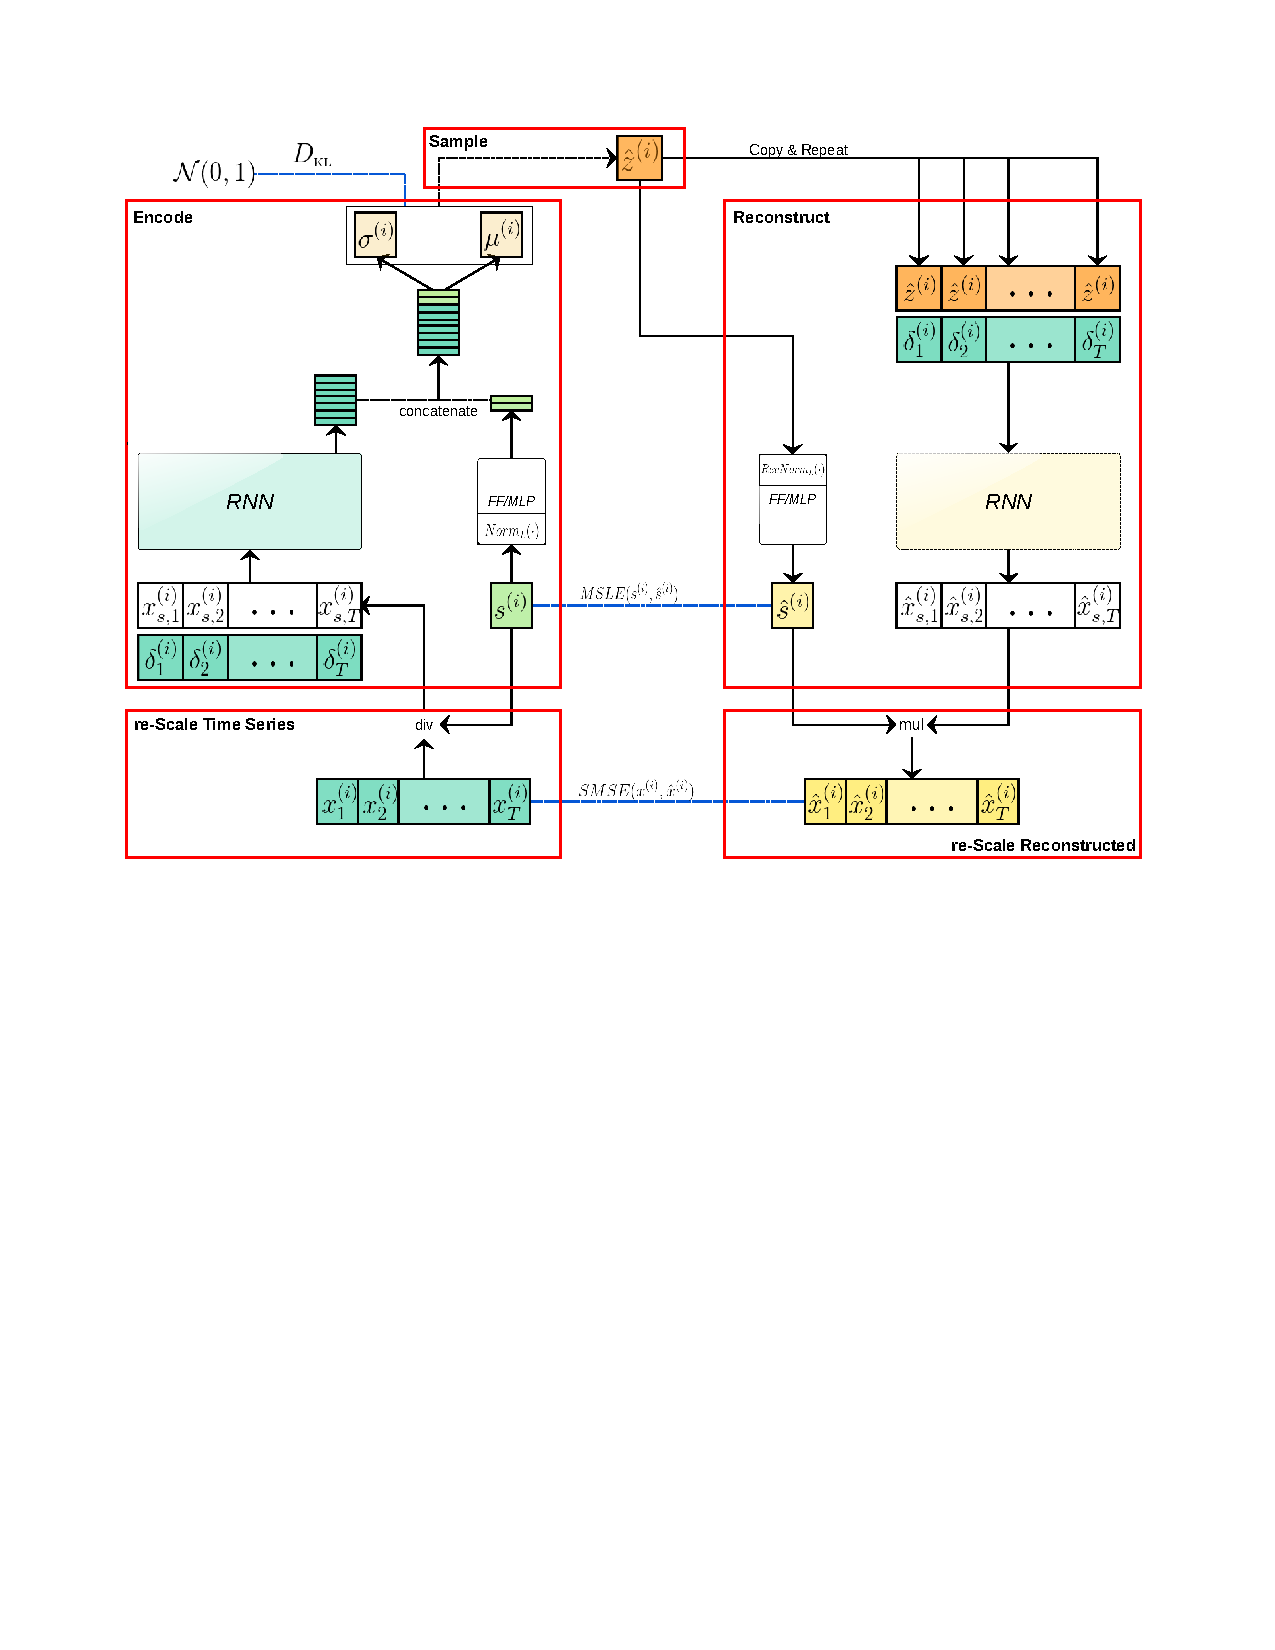
\includegraphics[width=\textwidth]{imgs/svrae_model.pdf}
    \caption{Diagram of the S-VRAE$_t$ architecture for irregularly sampled time series. Firstly, the raw time series input is re-scaled and pass to the RNN encoder block together with the delta times. In parallel the scale input is encoded too. A concatenation is perform on both learned embedding values to obtain the Normal distribution parameters of the latent variable. After a sample is performed over this distribution, the value is repeated and concatenated with the delta times in order to reconstruct the scaled time series and the original scale. Finally the raw scale is returned to the time series.}
    \label{arch:svrae_ill}
\end{figure}
The  architecture of the proposed \textbf{S-VRAE$_t$} is illustrated on Figure \ref{arch:svrae_ill}. Please note that the Encode and Reconstruct blocks are the same of the RAE$_t$ on Figure~\ref{arch:bnaul} but without the scale transformations. 
%BENEFICIOS/Ventajas/CONTRIBUCIONES
In summary, S-VRAE$_t$ learns a coded \textit{deep representation} of the unevenly-sampled raw time series in an unsupervised way. The advantage is that those features are optimized for the specific input behavior (rather than classification) and have less bias than human-crafted counterparts. The evidence for this claim can be found in Section \ref{res}.

%denoising -- era la motivacion original
In any VAE model, the objective of learning the distribution of the latent variable is to obtain the more likely reconstructed input pattern. In our S-VRAE$_t$ model the time series gets reconstructed on the original scale, $\hat{x}^{(i)}$, so we can consider it as a smoothing or denoising model on a data-dependent way (based on the data behavior).
As the model processes the scale inside it, allows to remove the noise inside the scale.
For example, consider a decomposition of the time series measurements based on $x^{(i)} =  x_p^{(i)} + n^{(i)}$, with $n^{(i)}$ the intrinsic noise of every measurement on $x_p^{(i)}$, and $x_p^{(i)}$ the time series measurements with isolated or perfect environment, as the one modeled by \citep{mandel2002analytic}. 
On this case, the denoised scale would be $s_p^{(i)} = std(x_p^{(i)})$ and could only be learned by S-VRAE$_t$ in order to re-scale the reconstructed denoised time series $\hat{x}_p^{(i)} = \hat{x}_{p,s}^{(i)}\cdot s_p^{(i)}$. 
Any other model with the re-scaling process fixed would use a noised scale, for example, $s^{(i)} = std(x^{(i)}) = std(x_p^{(i)} + n^{(i)})$.
This shows the capacity of S-VRAE$_t$ to denoise raw time series.
%based on the previous decomposition we can express the square of the scale (or the variance) by 
%$(s^{(i)})^2 = std(x^{(i)})^2 = var(x_p^{(i)} + n^{(i)})= var(x_p^{(i)}) +  var(n^{(i)}) + 2 cov(x_p^{(i)},n^{(i)}) $, with $cov$ the covariance.

%On the other hand, models like RAE$_t$ and VRAE$_t$ have to process (i.e., encode and reconstruct) the standardized version of the data $x_s^{(i)}$. Then, from outside the model the original scale could be returned, with the real value ($s^{(i)}$), this is $\hat{x}^{(i)} = \hat{x}_s^{(i)}\cdot s^{(i)}$. The problem is that there could be is noise inside the real scale, $s^{(i)} = std(x^{(i)}) \approx std(\check{x}^{(i)} + n^{(i)}) = std(\check{x}^{(i)}) +  std(n^{(i)}) $, with $n^{(i)}$ the intrinsic noise of every measurement on the time series $\check{x}^{(i)}$, and $\check{x}^{(i)}$ the time series measurement with isolated or perfect environment, as the one simulated by M-A model \citep{mandel2002analytic}.


%However, smoothing or denoising a light curve is not straightforward for transits, because the transits can be seen as isolated behaviors or anomalies (i.e., threshold events) as Figure \ref{fig:representation_ex} shows. Therefore, a \textit{vanilla} denoising model will remove transits by considering them anomaly deviations of the ``normal'' star magnitude.


%Optimization:
\subsection{Loss Function}
In this section we describe the optimization objectives of the Variational Auto-Encoder models (VRAE$_t$ and S-VRAE$_t$) for time series domain.

\textbf{Reconstruction loss} \ \ 
We use a modified version of the mean squared error (\textit{MSE}) loss function for time series, named \textit{weighted} or \textit{re-scaled} \textit{MSE}, given by
\begin{equation}
    SMSE(X, \hat{X}) = \frac{1}{N} \sum_{i=1}^N w^{(i)} \cdot \frac{1}{T_i} \sum_{j=1}^{T_i} \left( x_j^{(i)} - \hat{x}_j^{(i)}  \right)^2 \, ,
\end{equation}
where weight $w^{(i)}$ is associated to every input pattern (as a \textit{sample weight} \citep{freund1995desicion}) and is defined as the inverse to variance $w^{(i)} = 1/var(x^{(i)})$. The weight value is derived from $w_i = \left(1/s^{(i)}\right)^2$, with the idea of remove the intrinsic scale (standard deviation) of the time series $x^{(i)}$, and so every input pattern has the same impact on the objective. In order to perform a proper reconstruction of the input patterns, the SMSE would be the loss function of the deterministic counterpart of VRAE$_t$, this is, the RAE$_t$ model.

\textbf{Variational loss} \ \ The two factors to optimize on the variational lower bound (Equation \ref{eq:basic_obj}) could be expressed by: i) a reconstruction factor through the \textit{SMSE} described above, and ii) the closed solution of a \textit{KL} divergence with Normal priors \citep{kingma2013auto}.
%The Variational lower bound of Equation \ref{eq:basic_obj}, has two factors to optimize. The first factor (reconstruction) is expressed through the \textit{SMSE} described above, while the \textit{KL} divergence is expressed as the closed form solution with Normal priors distribution presented by \citep{kingma2013auto}. 
Following \citep{higgins2017beta}, we combine these two factors using a regularization parameter $\beta$ obtaining the loss function of the VRAE$_t$ model:
\begin{equation}
    V(X, \hat{X}) = SMSE(X, \hat{X}) + \beta \cdot KL(Z) \, .
\end{equation}
Our earlier experiments on validation set led us to set the $\beta$ parameter to a small value of $10^{-3}$. This mean that the priority is set on the reconstruction task but with a variational component.


\textbf{Variational loss with re-Scaling} \ \ As our proposed S-VRAE$_t$ adds the scale to the reconstruction task, we need to specify an additional loss for this. We used the mean squared logarithm error (\textit{MSLE}) as loss function, given by %to scale reconstruction:
\begin{equation}
MSLE(S, \hat{S}) = \frac{1}{N} \sum_{i=1}^N \left( \log{s^{(i)}} - \log{\hat{s}^{(i)}}  \right)^2 \, .
\end{equation}
Then, the learning objective of S-VRAE$_t$ model is given by:
\begin{equation}
    SV \left( (X,S) , (\hat{X},\hat{S}) \right)=  V(X, \hat{X}) + \alpha \cdot MSLE(S, \hat{S}) \, ,
\end{equation}
where the $\alpha$ parameter was set to $10^{-1}/var(\log{S})$. The same motivation used for $\beta$ led to set the $10^{-1}$ value, giving firstly relevance to the reconstruction loss \textit{SMSE} inside \textit{V}. While the $var(\log{S})$ value is to re-scale the magnitude of the \textit{MSLE} loss (by removing the standard deviation) to the same proportions of \textit{SMSE} loss.



